% One-asset moment match vignette (1--2 pages)
% Operationalizes Section 6.1: κ directly estimable; σr calibration target; φ=λση composite.
% Publication-safe: no unit-mismatched ση/λ comparison.

\subsection{One-asset moment match vignette}
\label{sec:moment_match_vignette}

We illustrate how the identification mapping in \S\ref{sec:param_identification} can be operationalized using a single liquid ETF (SPY).
Before turning to SPY-specific mapping and estimates, we report brief implementation checks under the baseline parameterization (particle convergence in $N$ and $\lambda$-sensitivity; Tables~\ref{tab:convergence}--\ref{tab:sensitivity}).

\paragraph{Units and mapping.}
One simulation step corresponds to one trading day; half-life in days maps directly to $\kappa$ per step.
The model \eqref{eq:anchored_impact} uses the \emph{price increment} $dp_t$ (i.e., $\Delta p$ in value units), not log returns $\Delta\log p$ or simple returns $\Delta p/p$.
Empirically, we work with log returns $\Delta\log P_t$; for small moves, $\Delta\log P_t \approx \Delta P_t/P_t$. We therefore use the linearization
$\Delta\log P_t \approx s\,\Delta p_t$ with $s:=1/\bar P$, where $\bar P$ is the sample mean price level (reported in Table~\ref{tab:spy_moment_match}).
Given this mapping, we calibrate the \emph{price-noise scale} $\phi$ in \eqref{eq:anchored_impact} to match $\sigma_r$ via $\sigma_r \approx s\,\phi$ (i.e., $\phi \approx \sigma_r/s$).
Identifying $\lambda$ itself requires an order-flow proxy; in this vignette we treat $\lambda$ as an external normalization and infer the implied order-flow noise scale mechanically as $\sigma_\eta=\phi/\lambda$ (Section~II, microstructure sketch).

From daily adjusted-close data (MacroTrends; \input{../paper_artifacts/moment_match/table_moment_match_n_obs.tex} trading days, \input{../paper_artifacts/moment_match/table_moment_match_start.tex}--\input{../paper_artifacts/moment_match/table_moment_match_end.tex}), we estimate:
(i) an anchoring/mean-reversion rate $\kappa$ from a half-life diagnostic, and
(ii) the unconditional return volatility $\sigma_r$ as a calibration target.

\paragraph{Audit-able estimation procedure.}
\ifjeicblind The estimation procedure (link omitted for blind review) implements the following, fully reproducible from the data. \else The script \texttt{code/scripts/estimate\_moment\_match.py} implements the following, fully reproducible from the data. \fi
(i) \textbf{Half-life conversion:} We use the canonical mapping \eqref{eq:half_life_conversion} between mean-reversion speed $\kappa$ and half-life $h$.
(ii) \textbf{Estimating $\kappa$ from the proxy mispricing series:} We form the relative mispricing proxy
$y_t := (P_t-\mathrm{MA}_t)/\mathrm{MA}_t$, where $\mathrm{MA}_t$ is a slow moving average (200-day, or $\min(200, n/4)$ for shorter series).
For small deviations, $y_t \approx \ln P_t - \ln(\mathrm{MA}_t)$ (linearization); the half-life diagnostic is invariant to scaling of $y_t$.
We fit the AR(1) model $y_t = \rho y_{t-1} + \varepsilon_t$ and obtain the half-life $h = -\ln(0.5)/\ln(\rho)$ days; then $\kappa = (\ln 2)/h$.
For SPY we obtain $h \approx \input{../paper_artifacts/moment_match/table_moment_match_hl.tex}$ days, hence $\kappa \approx \input{../paper_artifacts/moment_match/table_moment_match_kappa.tex}$ per trading day.
(iii) \textbf{Mapping $\sigma_r$ to $\phi$:} We use the realized daily log-return volatility $\sigma_r \approx \input{../paper_artifacts/moment_match/table_moment_match_sigma_r.tex}$ (annualized $\approx \input{../paper_artifacts/moment_match/table_moment_match_sigma_r_ann.tex}$) as a calibration target for $\phi$ under the linearization $\sigma_r \approx s\,\phi$ described above. Given an externally chosen $\lambda$, we then infer $\sigma_\eta=\phi/\lambda$.
Our model baseline uses $\kappa=0.005$ (half-life $\approx 139$ days), so SPY maps to a baseline/high-anchoring regime.

\begin{table}[t]
  \centering
  \scriptsize
  \caption{SPY moment match and regime classification (daily units).}
  \label{tab:spy_moment_match}
  \begin{tabular}{lccc}
    \toprule
    \textbf{Quantity} & \textbf{Estimate} & \textbf{Baseline} & \textbf{Notes} \\
    \midrule
    Anchoring rate $\kappa$ & \input{../paper_artifacts/moment_match/table_moment_match_kappa.tex} & \input{../paper_artifacts/moment_match/table_moment_match_kappa_baseline.tex} & $\kappa = (\ln 2)/h$ \\
    Half-life $h$ (days) & \input{../paper_artifacts/moment_match/table_moment_match_hl.tex} & \input{../paper_artifacts/moment_match/table_moment_match_hl_baseline.tex} & $h = (\ln 2)/\kappa$ \\
    Mean price $\bar P$ & \input{../paper_artifacts/moment_match/table_moment_match_mean_price.tex} & --- & used for $s:=1/\bar P$ \\
    Scale $s$ & \input{../paper_artifacts/moment_match/table_moment_match_scale_s.tex} & --- & $\Delta\log P\approx s\,\Delta p$ \\
    Return vol $\sigma_r$ & \input{../paper_artifacts/moment_match/table_moment_match_sigma_r.tex} & --- & daily log-return vol \\
    Price-noise $\phi$ & \input{../paper_artifacts/moment_match/table_moment_match_phi.tex} & \input{../paper_artifacts/moment_match/table_moment_match_phi_baseline.tex} & calibrated via $\sigma_r\approx s\,\phi$ \\
    Impact $\lambda$ & \input{../paper_artifacts/moment_match/table_moment_match_lambda_norm.tex} & \input{../paper_artifacts/moment_match/table_moment_match_lambda_norm.tex} & normalization (volume needed to estimate) \\
    Implied $\sigma_\eta=\phi/\lambda$ & \input{../paper_artifacts/moment_match/table_moment_match_sigma_eta_implied.tex} & \input{../paper_artifacts/moment_match/table_moment_match_sigma_eta_baseline.tex} & inferred mechanically \\
    \midrule
    \textbf{Regime} & \input{../paper_artifacts/moment_match/table_moment_match_regime.tex} & baseline & high anchoring \\
    \bottomrule
  \end{tabular}
\end{table}

\paragraph{Results.}
Table~\ref{tab:spy_moment_match} reports the moment match and regime classification.
\ifjeicblind The estimates are produced using the replication package. Link omitted for blind review. \else The estimates are produced by running \texttt{python code/scripts/estimate\_moment\_match.py --ticker SPY --csv <path>}; outputs are written to \texttt{paper\_artifacts/moment\_match/}. \fi
Figure~\ref{fig:moment_match_regime} plots the estimated $\kappa$ against the baseline and stress regions (regime is determined by anchoring strength $\kappa$).
SPY is in the \emph{baseline} regime with half-life $\approx \input{../paper_artifacts/moment_match/table_moment_match_hl.tex}$ trading days.
The daily return volatility $\sigma_r$ is a calibration target; under the unit mapping above, price-only data pin down $\phi$ while $\lambda$ requires an order-flow proxy, and then $\sigma_\eta=\phi/\lambda$ is inferred mechanically.

\paragraph{Why mispricing does not move with $k$: architecture bridge.}
Our model architecture explains why mispricing remains largely unchanged when increasing $k$ across the joint grid (Subsection~\ref{subsec:joint_grid}) and one-at-a-time sweeps (Subsection~\ref{subsec:sweeps}).
Overconfidence $k$ enters only through the Kalman filter (Appendix~A): it scales the perceived signal precision $R'_i = \sigma_\epsilon^2/k$, so higher $k$ yields tighter beliefs and more aggressive demand.
But the price dynamics \eqref{eq:anchored_impact} have two channels: (a) $\kappa(v_t-p_t)$ pulls the price toward fundamentals (arbitrage/anchoring), and (b) $\lambda\bar u_t$ reflects flow-based impact from trading rates.
Under strong anchoring (high $\kappa$), the $\kappa(v_t-p_t)$ term dominates: prices track fundamentals regardless of belief dispersion.
Thus $k$ loads mainly onto disagreement and trading intensity (belief dispersion, perceived precision, demand aggressiveness) rather than onto the price level itself.
This structural separation---$k$ shifts dispersion and intensity, whereas $(\kappa,\lambda,\phi)$ govern mispricing magnitudes---matches what we report in Tables~\ref{tab:metrics}--\ref{tab:joint_grid}.

\paragraph{Caveats.}
The fundamental $v_t$ is unobservable; the moving average is a rough proxy.

\begin{figure}[t]
  \centering
  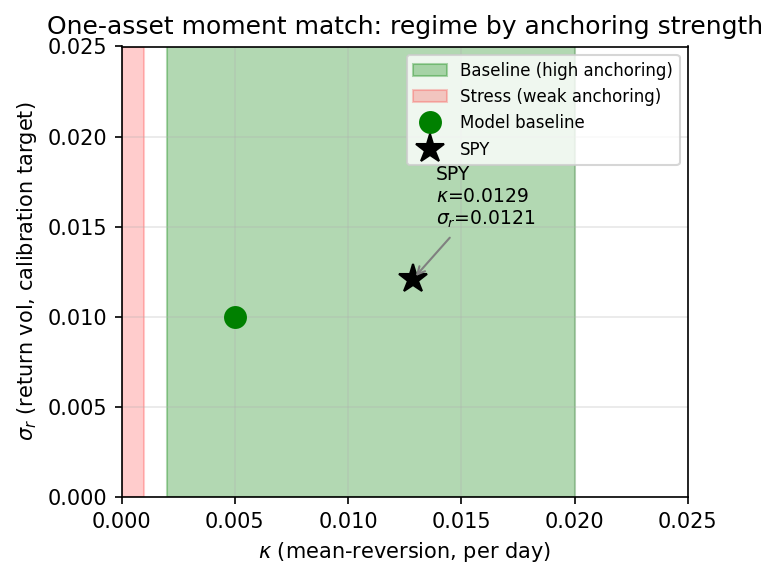
\includegraphics[width=0.48\textwidth]{../paper_artifacts/moment_match/fig_moment_match_regime.png}
  \caption{One-asset moment match: estimated $\kappa$ for SPY vs.\ baseline and stress regions (regime by anchoring strength). $\sigma_r$ shown as calibration target.}
  \label{fig:moment_match_regime}
\end{figure}
